%----------------------------------------------------------------------------------------
%	PACKAGES AND OTHER DOCUMENT CONFIGURATIONS
%----------------------------------------------------------------------------------------

\documentclass{article}

\usepackage{fancyhdr} % Required for custom headers
\usepackage{lastpage} % Required to determine the last page for the footer
\usepackage{extramarks} % Required for headers and footers
\usepackage{graphicx} % Required to insert images
\usepackage{amsmath, amssymb} % Required for Maths
\usepackage{mathtools} % Required for Maths
\usepackage{enumerate}
\usepackage{mathtools}
\usepackage{textcomp}
\usepackage{gensymb}
\usepackage{siunitx}
\usepackage{empheq}
\usepackage{ulem}
\usepackage{amssymb}

% Margins
\topmargin=-0.45in
\evensidemargin=0in
\oddsidemargin=0in
\textwidth=6.5in
\textheight=9.0in
\headsep=0.25in 

\linespread{1.1} % Line spacing

% Set up the header and footer
\pagestyle{fancy}
\lhead{\hmwkAuthorName} % Top left header
\chead{\hmwkClass\ (\hmwkClassInstructor\ \hmwkClassTime): \hmwkTitle} % Top center header
\rhead{\firstxmark} % Top right header
\lfoot{\lastxmark} % Bottom left footer
\cfoot{} % Bottom center footer
\rfoot{Page\ \thepage\ of\ \pageref{LastPage}} % Bottom right footer
\renewcommand\headrulewidth{0.4pt} % Size of the header rule
\renewcommand\footrulewidth{0.4pt} % Size of the footer rule

\setlength\parindent{0pt} % Removes all indentation from paragraphs

%----------------------------------------------------------------------------------------
%	DOCUMENT STRUCTURE COMMANDS
%	Skip this unless you know what you're doing
%----------------------------------------------------------------------------------------

% Header and footer for when a page split occurs within a problem environment
\newcommand{\enterProblemHeader}[1]{
\nobreak\extramarks{#1}{#1 continued on next page\ldots}\nobreak
\nobreak\extramarks{#1 (continued)}{#1 continued on next page\ldots}\nobreak
}

% Header and footer for when a page split occurs between problem environments
\newcommand{\exitProblemHeader}[1]{
\nobreak\extramarks{#1 (continued)}{#1 continued on next page\ldots}\nobreak
\nobreak\extramarks{#1}{}\nobreak
}

\setcounter{secnumdepth}{0} % Removes default section numbers
\newcounter{homeworkProblemCounter} % Creates a counter to keep track of the number of problems

\newcommand{\homeworkProblemName}{}
\newenvironment{homeworkProblem}[1][Problem \arabic{homeworkProblemCounter}]{ % Makes a new environment called homeworkProblem which takes 1 argument (custom name) but the default is "Problem #"
\stepcounter{homeworkProblemCounter} % Increase counter for number of problems
\renewcommand{\homeworkProblemName}{#1} % Assign \homeworkProblemName the name of the problem
\section{\homeworkProblemName} % Make a section in the document with the custom problem count
\enterProblemHeader{\homeworkProblemName} % Header and footer within the environment
}{
\exitProblemHeader{\homeworkProblemName} % Header and footer after the environment
}

\newcommand{\problemAnswer}[1]{ % Defines the problem answer command with the content as the only argument
\noindent\framebox[\columnwidth][c]{\begin{minipage}{0.98\columnwidth}#1\end{minipage}} % Makes the box around the problem answer and puts the content inside
}

\newcommand{\homeworkSectionName}{}
\newenvironment{homeworkSection}[1]{ % New environment for sections within homework problems, takes 1 argument - the name of the section
\renewcommand{\homeworkSectionName}{#1} % Assign \homeworkSectionName to the name of the section from the environment argument
\subsection{\homeworkSectionName} % Make a subsection with the custom name of the subsection
\enterProblemHeader{\homeworkProblemName\ [\homeworkSectionName]} % Header and footer within the environment
}{
\enterProblemHeader{\homeworkProblemName} % Header and footer after the environment
}

%----------------------------------------------------------------------------------------
%	NAME AND CLASS SECTION
%----------------------------------------------------------------------------------------

\newcommand{\hmwkTitle}{Homework\ \#4} % Assignment title
\newcommand{\hmwkDueDate}{Wednesday,\ November\ 25,\ 2015} % Due date
\newcommand{\hmwkClass}{ENPM 808M} % Course/class
\newcommand{\hmwkClassTime}{4:00 PM} % Class/lecture time
\newcommand{\hmwkClassInstructor}{Dr. William Levine} % Teacher/lecturer
\newcommand{\hmwkAuthorName}{Kanishka Ganguly} % Your name

%----------------------------------------------------------------------------------------
%	TITLE PAGE
%----------------------------------------------------------------------------------------

\title{
\vspace{2in}
\textmd{\textbf{\hmwkClass:\ \hmwkTitle}}\\
\normalsize\vspace{0.1in}\small{Due\ on\ \hmwkDueDate}\\
\vspace{0.1in}\large{\textit{\hmwkClassInstructor\ \hmwkClassTime}}
\vspace{3in}
}

\author{\textbf{\hmwkAuthorName}}
\date{} % Insert date here if you want it to appear below your name

%----------------------------------------------------------------------------------------

\begin{document}

\maketitle

%----------------------------------------------------------------------------------------
%	TABLE OF CONTENTS
%----------------------------------------------------------------------------------------

%\setcounter{tocdepth}{1} % Uncomment this line if you don't want subsections listed in the ToC

\newpage
\tableofcontents
\newpage

%----------------------------------------------------------------------------------------
%	PROBLEM 1
%----------------------------------------------------------------------------------------
\begin{homeworkProblem}
\begin{homeworkSection}{(a)}
We have given that the desired trajectory begins at $q_i(0) = 0$ and ends at $q_i(5) = 15 \degree$. It is also given that $\dot q_i(0) = 0$ and $\dot q_i(5) = 0$.\\
Now, let us assume that the cubic polynomial is of the form $ax^3 + bx^2 + cx + d = q(t)$, say.
We thus have 4 conditions and 4 unknowns to solve.\\
\begin{align}
q(0) = 0\\
\implies d = 0\nonumber\\
q(5) = 15\\
\implies 5^3 a + 5^2 b + 5 c +d = 15\nonumber\\
\dot q(0) = 0\\
\implies c = 0\nonumber\\
\dot q(5) = 0\\
\implies 5^2.3 a + 2.5 b + c = 15\nonumber
\shortintertext{Solving above equations simultaneously, we get}\nonumber\\
q(t) = -\frac{6}{25}t^3 + \frac{9}{25}t^2
\end{align}
\end{homeworkSection}

\begin{homeworkSection}{(b)}
\problemAnswer{ % Answer
\begin{center}
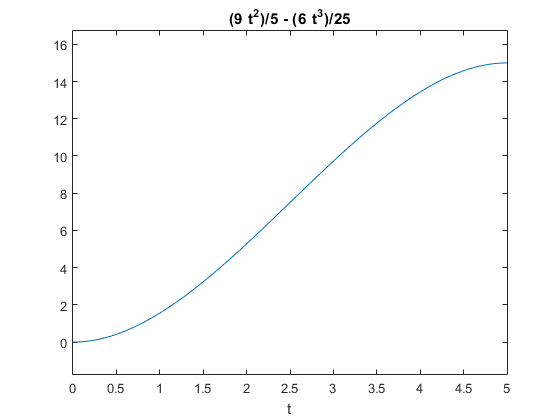
\includegraphics[width=0.75\columnwidth]{img/Q1.png}
\end{center}
}
\vspace{20pt}
Plot of Trajectory From 0 to 5
\end{homeworkSection}
\end{homeworkProblem}

%----------------------------------------------------------------------------------------
%	PROBLEM 2
%----------------------------------------------------------------------------------------
\begin{homeworkProblem} 
We have the following formula for an artificial potential function:
\begin{align}
U(q) = U_{att}(q) + U_{rep}(q)\label{eq:potential}\\
\shortintertext{where}\nonumber\\
U_{att}(q) =
\begin{cases}
\frac{1}{2} \zeta \rho^2_f(q) & :\quad\rho_f(q) \leq d\\\\
d\zeta \rho_f(q)-\frac{1}{2} \zeta d^2 & :\quad\rho_f(q) > d
\end{cases}\label{eqn:att}
\shortintertext{and where}\nonumber\\
U_{rep}(q) =
\begin{cases}
\frac{1}{2} \eta \Big(\frac{1}{\rho(q)} - \frac{1}{\rho_0} \Big)^2 & :\quad\rho_f(q) \leq \rho_0\\\\
0 & :\quad\rho_f(q) > \rho_0
\end{cases}\label{eqn:rep}
\end{align}

Also consider the following visual representation of the warehouse:\\
\problemAnswer{ % Answer
\begin{center}
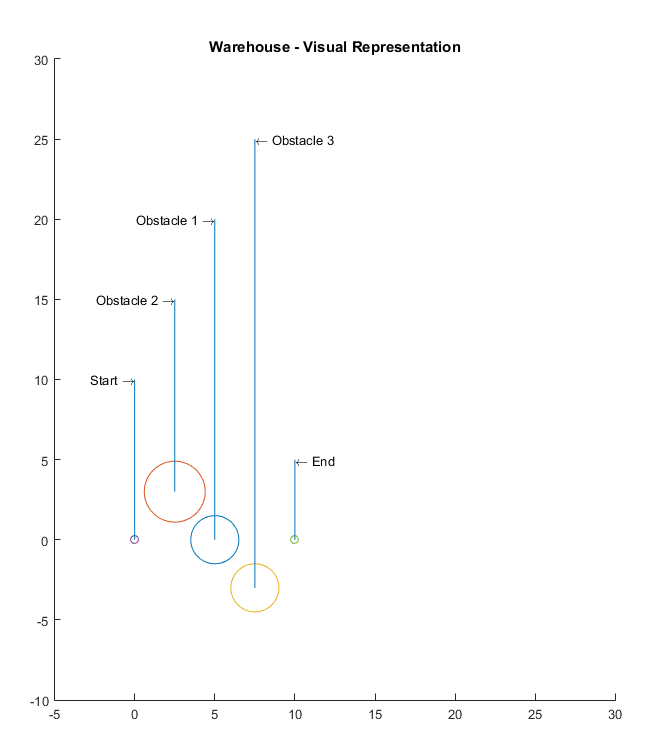
\includegraphics[width=0.6\columnwidth]{img/Q2.png}
\end{center}
}
\vspace{20pt}
Warehouse Representation

\begin{homeworkSection}{(a)}
Now, let the position of the center of the robot be $q \equiv (x,y)$. Consider the attractive potential formula from Eqn.~\ref{eqn:att}.\\
Here we have $\rho_f(q)$ as the Euclidean distance between the robot's center $q$ and the final destination $q_{\text{final}}$. Also, $\zeta$ represents a `scaling factor' for the attractive potential.\\
Let us assume that $d=2$ and $\zeta = 10$. Then, for the two cases, we have:
\begin{align}
U_{att}(q) =
\begin{cases}
\frac{1}{2}\times10\times\Big(\sqrt{(x-10)^2 + y^2} \Big)^2 & :\quad\rho_f(q) \leq 2\\\\
2 \times 10 \Big(\sqrt{(x-10)^2 + y^2} \Big)^2 -\frac{1}{2} \times 10 \times 4 & :\quad\rho_f(q) > 2
\end{cases}\\\\
\implies
U_{att}(q) =
\begin{cases}
5\times\Big(\sqrt{(x-10)^2 + y^2} \Big)^2 & :\quad\rho_f(q) \leq 2\\\\
5\times\Big(\sqrt{(x-10)^2 + y^2} \Big)^2 - 20 & :\quad\rho_f(q) > 2
\end{cases}
\end{align}
The reason for choosing a relatively high value for $\zeta$ is that \textit{(from Fig.)} between obstacles 1 and 3, there is a possibility that the repulsive forces $U_{rep}1$ and $U_{rep}3$ together can be larger than the attractive potential $U_{att}$.\\
This will mean that the robot will never be able to pass through these two obstacles towards the final destination.\\
Thus, by having $\zeta = 10$, we can ensure that that the attractive force is sufficiently high for the robot to overcome the local minimal potential and move towards global attractive potential.\\

Next, we consider the repulsive potential fields produced by each of the obstacles. It must be noted that each of the obstacles has a projected radius of 1 m. However, the `effective' potential radius of the obstacles must be decided carefully to prevent local minima.\\
The obstacles 1 and 2 \textit{(from Fig.)} are arranged such that there might be a situation where, as the robot reaches the potential field of obstacle 2, it is also in the potential field of obstacle 1.\\
This will mean that when a local minima is reached (when attractive potential equals repulsive potential), the robot will simply get `stuck' in a potential well and will not find a way out towards the final destination.\\
To prevent such a situation from occurring, we must ensure that the potential field of obstacle 2 is large enough to cause a slight `imbalance' in potentials and `push' the robot downwards and away from this local minima.\\
We now calculate the actual repulsive potentials for each obstacle as given in Eqn.~\ref{eqn:rep}. Let $\rho(q)$ be defined as the minimum distance between the boundary of obstacle to boundary of robot. The center of the robot is given by $C \equiv (x,y)$.
So, we have:
\begin{align}
\rho(q) = distance(\text{center(robot)}, \text{center(obstacle)}) - sum(\text{radius(obstacle)}, \text{radius(robot)})
\end{align}
Calculating $U_{rep}1$ for obstacle at $O_1(5,0)$
\begin{align}
U_{rep}1 =
\begin{cases}
\frac{1}{2}\times\Big(\frac{1}{\sqrt{(x-5)^2 + y^2}-1.5} - 1 \Big)^2 & :\quad\rho(q) \leq 1\\\\
0 & :\quad\rho(q) > 1
\end{cases}
\end{align}
Calculating $U_{rep}2$ for obstacle at $O_2(2.5,3)$
\begin{align}
U_{rep}2 =
\begin{cases}
\frac{1}{2}\times\Big(\frac{1}{\sqrt{(x-2.5)^2 + (y-3)^2}-1.5} - \frac{1}{1.2} \Big)^2 & :\quad\rho(q) \leq 1.2\\\\
0 & :\quad\rho(q) > 1.2
\end{cases}
\end{align}
Calculating $U_{rep}3$ for obstacle at $O_3(7.5,-3)$
\begin{align}
U_{rep}3 =
\begin{cases}
\frac{1}{2}\times\Big(\frac{1}{\sqrt{(x-7.5)^2 + (y+3)^2}-1.5} - 1 \Big)^2 & :\quad\rho(q) \leq 1\\\\
0 & :\quad\rho(q) > 1
\end{cases}
\end{align}
In all three cases, the value of $\eta$ is taken as $\eta = 1$.

In conclusion, the artificial potential function is given from Eqn.~\ref{eq:potential} as:
\begin{align}
U(q) = U_{att} + U_{rep}1 + U_{rep}2 + U_{rep}3
\end{align}
\end{homeworkSection}

\begin{homeworkSection}{(b)}
Given a potential field $U$ we have the force exerted by the field as $F = -\nabla U$. Decomposing into components, we get $F_x = \frac{\partial U}{\partial x}$ and $F_y = \frac{\partial U}{\partial y}$.\\
Here,
\begin{align}
F_{rep}(q) =
\begin{cases}
\eta \Big(\frac{1}{\rho(q)} - \frac{1}{\rho_0} \Big) \frac{1}{\rho^2(q)} \nabla\rho(q) & :\quad\rho_f(q) \leq \rho_0\\\\
0 & :\quad\rho_f(q) > \rho_0
\end{cases}\label{eqn:Frep}
\end{align}

Considering obstacle 1,
\begin{align}
F_{rep}1_x = 
\begin{cases}
-\Bigg(\frac{1}{\sqrt{(x-5)^2 + y^2}-1.5}-1\Bigg)\times-\frac{1}{2}\frac{\Big[ \big((x-5)^2+y^2\big)^\frac{3}{2} (2x - 10)\Big]}{({\sqrt{(x-5)^2 + y^2}-1.5})^2} & :\quad\rho(q) \leq 1\\\\
0 & :\quad\rho(q) > 1
\end{cases}\\
F_{rep}1_y = 
\begin{cases}
-\Bigg(\frac{1}{\sqrt{(x-5)^2 + y^2}-1.5}-1\Bigg)\times-\frac{1}{2}\frac{\Big[ \big((x-5)^2+y^2\big)^\frac{3}{2} (2y)\Big]}{({\sqrt{(x-5)^2 + y^2}-1.5})^2} & :\quad\rho(q) \leq 1\\\\
0 & :\quad\rho(q) > 1
\end{cases}
\end{align}

Considering obstacle 2,
\begin{align}
F_{rep}2_x = 
\begin{cases}
-\Bigg(\frac{1}{\sqrt{(x-2.5)^2 + (y-3)^2}-1.5}-\frac{1}{1.2}\Bigg)\times-\frac{1}{2}\frac{\Big[ \big((x-2.5)^2+(y-3)^2\big)^\frac{3}{2} (2x - 5)\Big]}{({\sqrt{(x-2.5)^2 + (y-3)^2}-1.5})^2} & :\quad\rho(q) \leq 1.2\\\\
0 & :\quad\rho(q) > 1.2
\end{cases}\\
F_{rep}2_y = 
\begin{cases}
-\Bigg(\frac{1}{\sqrt{(x-2.5)^2 + (y-3)^2}-1.5}-\frac{1}{1.2}\Bigg)\times-\frac{1}{2}\frac{\Big[ \big((x-2.5)^2+(y-3)^2\big)^\frac{3}{2} (2y-6)\Big]}{({\sqrt{(x-2.5)^2 + (y-3)^2}-1.5})^2} & :\quad\rho(q) \leq 1.2\\\\
0 & :\quad\rho(q) > 1.2
\end{cases}
\end{align}

Considering obstacle 3,
\begin{align}
F_{rep}3_x = 
\begin{cases}
-\Bigg(\frac{1}{\sqrt{(x-7.5)^2 + (y+3)^2}-1.5}-1\Bigg)\times-\frac{1}{2}\frac{\Big[ \big((x-7.5)^2+(y+3)^2\big)^\frac{3}{2} (2x - 15)\Big]}{({\sqrt{(x-7.5)^2 + (y+3)^2}-1.5})^2} & :\quad\rho(q) \leq 1\\\\
0 & :\quad\rho(q) > 1
\end{cases}\\
F_{rep}3_y = 
\begin{cases}
-\Bigg(\frac{1}{\sqrt{(x-7.5)^2 + (y+3)^2}-1.5}-1\Bigg)\times-\frac{1}{2}\frac{\Big[ \big((x-7.5)^2+(y+3)^2\big)^\frac{3}{2} (2y - 6)\Big]}{({\sqrt{(x-7.5)^2 + (y+3)^2}-1.5})^2} & :\quad\rho(q) \leq 1\\\\
0 & :\quad\rho(q) > 1
\end{cases}
\end{align}

Now we consider the force exerted by the attractive field $U_{att}$. This force, also decomposed into components, gives us $F_{att_x} = -\frac{\partial U_{att}}{\partial x}$ and $F_{att_y} = -\frac{\partial U_{att}}{\partial y}$.\\
Thus, we have:

\begin{align}
F_{att_x} =
\begin{cases}
5\times \frac{1}{2} \times \big( (x-10)^2 + y^2 \big)^\frac{-1}{2} (2x - 20) & : \quad\rho_f(q) \leq 2\\\\
10\times \big((x-10)^2 + y^2\big)^\frac{-1}{2} (2x-20) & :\quad\rho_f(q) > 2
\end{cases}\\
F_{att_y} =
\begin{cases}
5\times \frac{1}{2} \times \big( (x-10)^2 + y^2\big)^\frac{-1}{2} (2y) & :\quad \rho_f(q) \leq 2\\\\
10\times \big((x-10)^2 + y^2\big)^\frac{-1}{2} (2y) & :\quad\rho_f(q) > 2
\end{cases}
\end{align}

It is given in the problem statement that the dynamics of the robot are given by:
\begin{align}
m
\begin{bmatrix}
\ddot x(t)\\
\ddot y(t)
\end{bmatrix}
=
\begin{bmatrix}
F_x\\
F_y
\end{bmatrix}
\end{align}
with $m = 1\enspace$kilogram.

Thus, in conclusion, we have:
\begin{align}
\ddot x(t) = F_{total_x} = F_{att_x} + F_{rep}1_x + F_{rep}2_x + F_{rep}3_x\\
\ddot y(t) = F_{total_y} = F_{att_y} + F_{rep}1_y + F_{rep}2_y + F_{rep}3_y
\end{align}
\end{homeworkSection}
\end{homeworkProblem}
%----------------------------------------------------------------------------------------
%	PROBLEM 3
%----------------------------------------------------------------------------------------
\begin{homeworkProblem}
\problemAnswer{ % Answer
\begin{center}
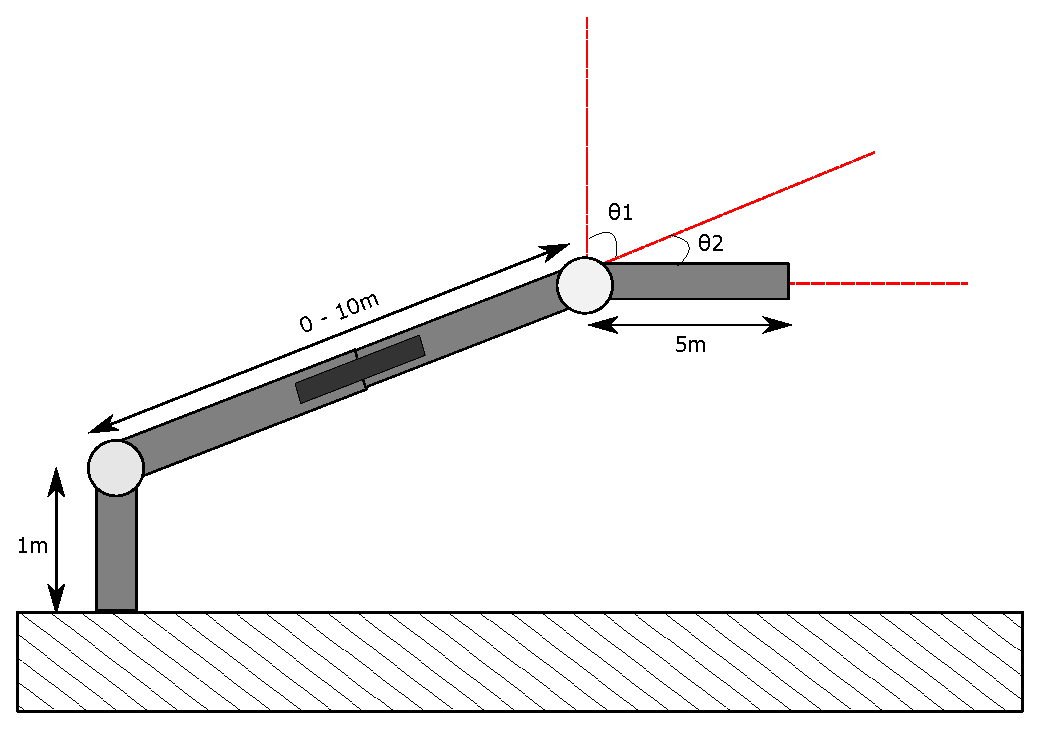
\includegraphics[width=0.6\columnwidth]{img/Q3a.eps}
\end{center}
}
\vspace{20pt}
Robot Diagram - Assumptions

The configuration space for a robot is defined as the collection (or space) of all possible configurations of the robot. Here a configuration is a specification of the position of every point on the robot.\\
To simplify our understanding and for easier calculations, consider the robot given in figure above as three separate portions.
\begin{itemize}
\item \textbf{The base}, from the reference to the first revolute joint.
\item \textbf{The `extendable' link}, from the first revolute joint to the second revolute joint.
\item \textbf{The last link}, from the second revolute joint.
\end{itemize}

Now, given these parts, we can develop a set of constraints of $\theta_1$ and $\theta_2$ with respect to links $L_1,L_2$ and $L_3$. The combination of these constraints will give us the set of all possible configurations of the robot, i.e. the configuration space.\\
Here, we make the basic assumption that the first revolute joint, at a distance of $1\enspace$m from the reference plane can rotate a complete 360\degree. \\\\
Consider the prismatic joint $L_2$, which can extend from $1\enspace$m to $10\enspace$m.\\
\problemAnswer{ % Answer
\begin{center}
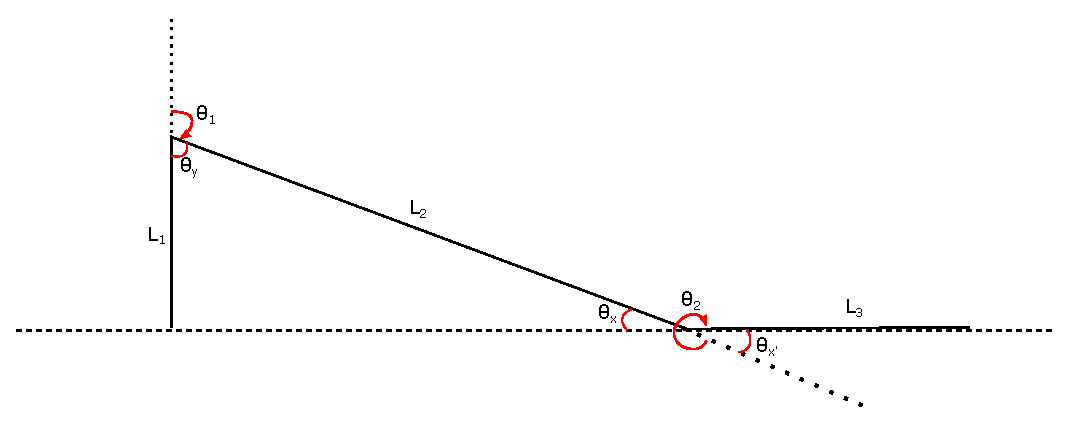
\includegraphics[width=0.8\columnwidth]{img/Q3-1.eps}
\end{center}
}
\vspace{20pt}
Robot Diagram - Link $L_2$

We now have the following equations based on diagram above:
\begin{align}
\theta_x = \theta_{x^\prime} = sin^{-1}\Big(\frac{L_1}{L_2} \Big)\\
\theta_y = 180\degree - \big( 90\degree + sin^{-1}\Big(\frac{L_1}{L_2} \Big) \big)\\
\theta_1 = 90\degree + sin^{-1}\Big(\frac{L_1}{L_2} \Big)\\
\theta_2 = 360\degree - sin^{-1}\Big(\frac{L_1}{L_2} \Big)\\
\shortintertext{Thus,}\nonumber\\
\implies sin(\theta_1 - 90\degree) = \frac{1}{L_2}\\
\implies sin(\theta_2 - 360\degree) = \frac{1}{L_2}
\end{align}

Consider the link $L_3$ attached to the revolute joint, which is of length $5\enspace$m.\\
\problemAnswer{ % Answer
\begin{center}
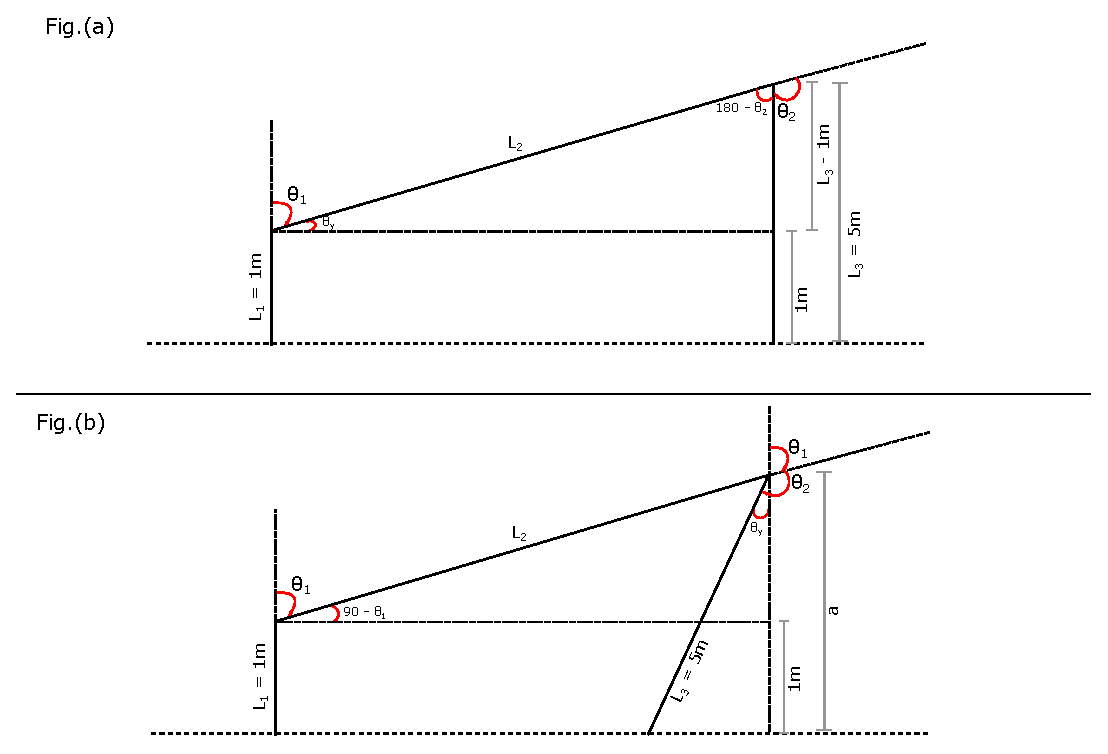
\includegraphics[width=0.8\columnwidth]{img/Q3-2.eps}
\end{center}
}
\vspace{20pt}
Robot Diagram - Link $L_3$

Taking Fig.(a), where $L_3$ is perpendicular to the reference, we have:
\begin{align}
sin(\theta_y) = \frac{L_3 - 1}{L_2}\\
\implies 90-\theta_1 = sin^{-1}\Big(\frac{L_3 - 1}{L_2}\Big)\\
\shortintertext{Also,}\nonumber\\
(180\degree - \theta_2) + (90\degree - \theta_1) = 90\degree\\
\implies (180\degree - \theta_2) + sin^{-1}\Big(\frac{L_3 - 1}{L_2}\Big) = 90\degree\\
\shortintertext{Thus,}\nonumber\\
\implies sin(90\degree - \theta_2) = sin^{-1}\Big(\frac{L_3 - 1}{L_2}\Big)\\
\implies sin(90\degree - \theta_1) = sin^{-1}\Big(\frac{L_3 - 1}{L_2}\Big)
\end{align}

Taking Fig.(b), where $L_3$ makes any other angle to the reference, we have:
\begin{align}
\theta_y = \theta_1 + \theta_2 - 180\degree\\
a = L_2 cos(90\degree - \theta_1) + L_1\\
cos(\theta_y) = L_2 cos(\theta_1) + L_1\\
\shortintertext{Thus,}\nonumber\\
\implies cos(\theta_1 + \theta_2 - 180\degree) = \frac{L_2 cos(\theta_1) + L_1}{L_3}
\end{align}

Thus, in conclusion, we have a set of equations that provide us with all the possible configurations of the robot in the workspace. The configuration space can thus be written as the following set of equations:
\begin{itemize}
\item
$cos(\theta_1 + \theta_2 - 180\degree) = \frac{L_2 cos(\theta_1) + L_1}{L_3}$
\item
$sin(90\degree - \theta_2) = sin^{-1}\Big(\frac{L_3 - 1}{L_2}\Big)$
\item
$sin(90\degree - \theta_1) = sin^{-1}\Big(\frac{L_3 - 1}{L_2}\Big)$
\item
$sin(\theta_1 - 90\degree) = \frac{1}{L_2}$
\item
$sin(\theta_2 - 360\degree) = \frac{1}{L_2}$
\end{itemize}
\end{homeworkProblem}

\end{document}